\documentclass[tikz,crop]{standalone}
\usepackage{fontspec}
\usepackage{unicode-math}
\setmainfont{STIX Two Text}
\setmathfont{STIX Two Math}
\usepackage{tikz}
\usepackage{pgfplots}
\pgfplotsset{compat=1.18}
\usetikzlibrary{arrows.meta,calc,positioning}

\begin{document}
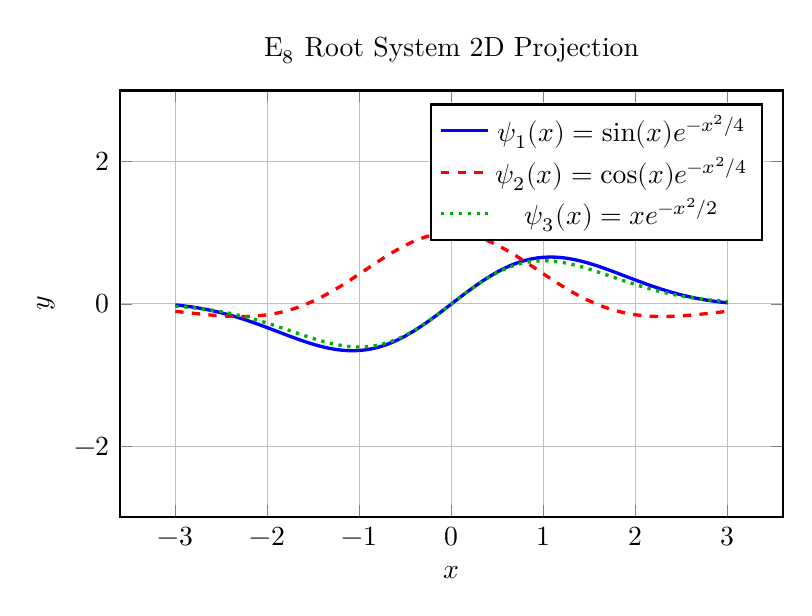
\begin{tikzpicture}
  \begin{axis}[
    width=10cm, height=7cm,
    xlabel={$x$},
    ylabel={$y$},
    title={E$_8$ Root System 2D Projection},
    grid=both,
    thick,
    samples=100,
    domain=-3:3,
    ymin=-3, ymax=3,
    legend pos=north east
  ]
    % Plot some example curves representing E8 symmetry projections
    \addplot[blue, very thick] {sin(deg(x)) * exp(-x^2/4)};
    \addlegendentry{$\psi_1(x) = \sin(x) e^{-x^2/4}$}

    \addplot[red, very thick, dashed] {cos(deg(x)) * exp(-x^2/4)};
    \addlegendentry{$\psi_2(x) = \cos(x) e^{-x^2/4}$}

    \addplot[green!70!black, very thick, dotted] {x * exp(-x^2/2)};
    \addlegendentry{$\psi_3(x) = x e^{-x^2/2}$}
  \end{axis}
\end{tikzpicture}
\end{document}
